%\documentclass{article}
%\usepackage{graphicx,subfigure}
%\begin{document}

\begin{figure}[!h]
  \centering
  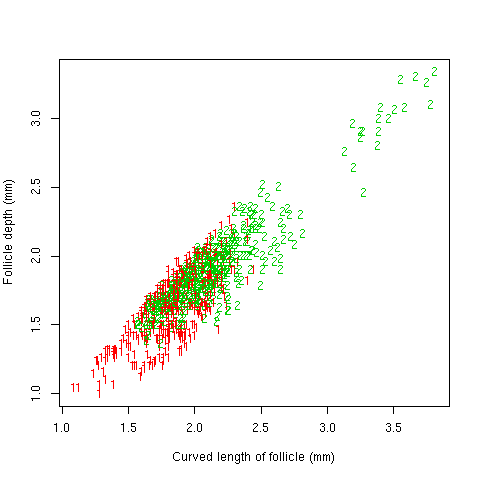
\includegraphics[width=1.0\textwidth]{curvlenxfd.png}
  \caption{Plot of follicle depth against curved length of follicles. The loose and wrinkly skintypes are shown as points labelled 1 ( red) and 2(green) respectively.}
  \label{fig:curvlenxfd}
\end{figure}

%\end{document}

